\section{Análise sintática preditiva não-recursiva}

\begin{frame}[fragile]{Analisador preditivo não-recursivo}

    \begin{itemize}
        \item É possível construir um analisador sintático preditivo não-recursivo, no qual as chamadas recursivas são eliminadas por meio do uso de uma
            pilha explícita
        \pause

        \item Seja recursivo ou não, o principal problema a ser resolvido por um analisador sintático é o de identificar a produção que deve ser aplicada a
            um não-terminal
        \pause

        \item Um analisador sintático não-recursivo busca em uma tabela sintática pela produção a ser aplicada
        \pause

        \item Tal tabela pode ser construída diretamente a partir de certas gramáticas
    \end{itemize}

\end{frame}

\begin{frame}[fragile]{Modelo de um analisador sintático preditivo não-recursivo}

    \begin{figure}
        \centering
        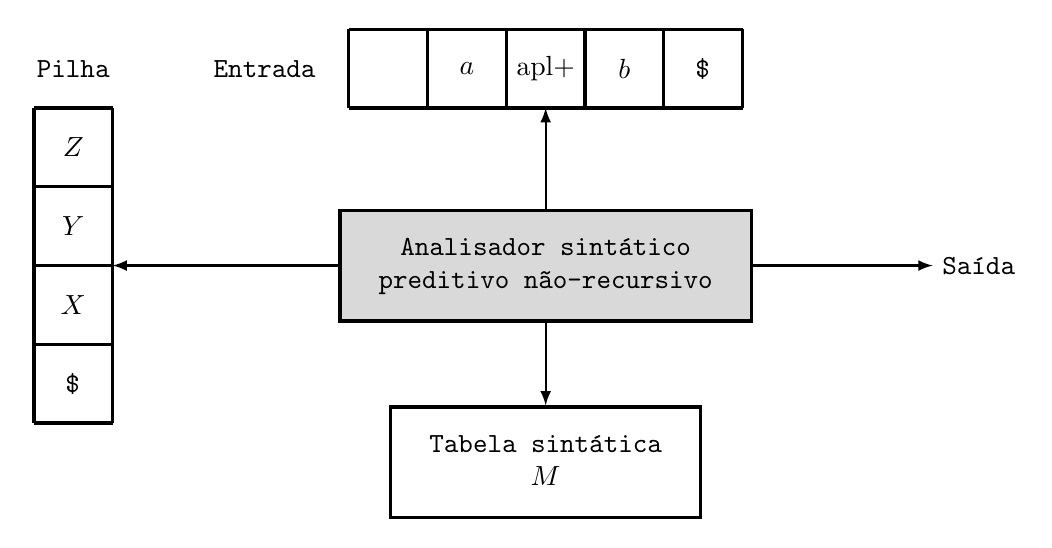
\begin{tikzpicture} 
            \node[draw,very thick,fill=gray!30,inner sep=8pt] (A) at (6.5, 3) { \texttt{\begin{tabular}{c} Analisador sintático\\ preditivo não-recursivo\end{tabular}} };
            \node[draw,very thick,inner sep=8pt] (B) at (6.5, 0.5) { \texttt{\begin{tabular}{c} Tabela sintática\\ $M$\end{tabular}} };
            \draw[very thick] (4, 5) grid (9, 6);
            \draw[very thick] (0, 1) grid (1, 5);

            \node (C) at (12, 3) { \texttt{Saída} };

            \node[anchor=east] at (3.7, 5.5) { \texttt{Entrada} };
            \node at (0.5, 5.5) { \texttt{Pilha} };

            \node at (0.5, 1.5) { \texttt{\$} };
            \node at (0.5, 2.5) { $X$ };
            \node at (0.5, 3.5) { $Y$ };
            \node at (0.5, 4.5) { $Z$ };

            \node at (5.5, 5.5) { $a$ };
            \node at (6.5, 5.5) { \code{apl}{+} };
            \node at (7.5, 5.5) { $b$ };
            \node at (8.5, 5.5) { \texttt{\$} };

            \draw[thick,-latex] (A) to (B);
            \draw[thick,-latex] (A) to (6.5, 5);
            \draw[thick,-latex] (A) to (1, 3);
            \draw[thick,-latex] (A) to (C);
        \end{tikzpicture} 
    \end{figure}

\end{frame}

\begin{frame}[fragile]{Estrutura de um analisador sintático preditivo não-recursivo}

    \begin{itemize}
        \item Um analisador sintático preditivo não-recursivo é composto por um \textit{buffer} de entrada, uma pilha, uma tabela sintática e um fluxo de saída
        \pause

        \item O \textit{buffer} de entrada contém a cadeia a ser analisada, seguida de um sentinela que indique o fim da cadeia (assuma que o sentinela é o
            caractere \texttt{\$})
        \pause

        \item A pilha contém símbolos gramaticais, um o sentinela indicando o fundo da pilha
        \pause

        \item Inicialmente a pilha deve contém o símbolo de partida da gramática logo acima do sentinela
        \pause
    
        \item A tabela sintática é uma matriz $M[A, a]$ cuja primeira dimensão contém não-terminais $A$ e a segunda contém terminais $a$ ou o sentinela
            \texttt{\$}
    \end{itemize}

\end{frame}

\begin{frame}[fragile]{Algoritmo para o analisar sintático preditivo não-recursivo}

    \begin{algorithmic}[1]
        \Require{Uma cadeia $w$ e uma tabela sintática $M$ para uma gramática $G$}
        \Ensure{Se $w\in L(G)$, uma derivação mais à esquerda de $w$, caso contrário sinaliza um erro}

        \vspace{0.1in}

        \State{$a\gets$ primeiro símbolo de $w$}
        \Repeat
            \State{$X\gets$ topo da pilha}
            \If{$X$ é um terminal}
                \If{$X = a$}
                    \State{remova $X$ da pilha}
                    \State{$a\gets$ próximo símbolo de $w$}
                \Else
                    \State{sinalize um erro}
                \EndIf
            \algstore{bkbreak}
    \end{algorithmic}

\end{frame}

\begin{frame}[fragile]{Algoritmo para o analisar sintático preditivo não-recursivo}

    \begin{algorithmic}[10]
        \algrestore{bkbreak}
            \ElsIf{$X$ é um não-terminal}
                \If{$M[A, a] = X \to Y_1Y_2\ldots Y_k$}
                    \State{remova $X$ da pilha}
                    \State{empilhe $Y_k, Y_{k - 1}, \ldots, Y_1$, com $Y_1$ no topo da pilha}
                    \State{escreva a produção $X \to Y_1Y_2\ldots Y_k$ na saída}
                \Else
                    \State{sinalize um erro}
                \EndIf
            \EndIf
        \Until{$X = $ \texttt{\$}}
    \end{algorithmic}

\end{frame}

\begin{frame}[fragile]{Tabela sintática para a gramática de expressões aritméticas}

    \begin{table}
        \centering
        \begin{tabular}{c|c|c|c|c|c|c}
        \toprule
        \multirow{2}{*}{\texttt{\begin{tabular}{c}Não-\\ terminal\end{tabular}}} & \multicolumn{6}{c}{\texttt{Símbolo da entrada}} \\
        \cmidrule{2-7}
        & \textbf{id} & \code{apl}{+} & \code{apl}{×} & $($ & $)$ & \texttt{\$} \\
        \midrule
        $E$ & $E\to TE'$ & & & $E\to TE'$ & \\
        \rowcolor[gray]{0.9}
        $E'$ & & $E'\to \code{apl}{+}TE'$ & & & $E'\to \code{apl}{∊}$ & $E'\to \code{apl}{∊}$ \\
        $T$ & $T\to FT'$ & & & $T\to FT'$ & \\
        \rowcolor[gray]{0.9}
        $T'$ & & $T'\to \code{apl}{∊}$ & $T'\to FT'$ & & $T'\to \code{apl}{∊}$ & $T'\to \code{apl}{∊}$ \\
        $F$ & $F\to \textbf{id}$ & & & $F\to (E)$ & & \\
        \bottomrule
        \end{tabular}
    \end{table}

\end{frame}

\begin{frame}[fragile]{Comportamento do analisador preditivo não-recursivo para a cadeia ``$\textbf{id}\code{apl}{+}\textbf{id}\code{apl}{×}\textbf{id}$''}

    \begin{tikzpicture}
        \node[opacity=0] at (12, 0) { . };
        \node[opacity=0] at (12, 7) { . };

        \node at (2.5, 0.5) { \texttt{Pilha} };

        \draw[very thick] (1.5, 1) to (3.5, 1);

        \draw[thick] (2, 1) rectangle (3, 2);
        \node at (2.5, 1.5) { \texttt{\$} };

        \draw[thick] (2, 2) rectangle (3, 3);
        \node at (2.5, 2.5) { $E$ };

        \node[anchor=west] at (5, 5) { \texttt{Entrada} };

        \node[anchor=west] at (6, 4) { \textbf{id} \code{apl}{+} \textbf{id} \code{apl}{×} \textbf{id} \texttt{\$} };

        \node[anchor=west] at (10, 5) { \texttt{Saída} };

%        \node[anchor=west] at (11, 4) { $E'\to \code{apl}{+}TE'$ };
    \end{tikzpicture}

\end{frame}

\begin{frame}[fragile]{Comportamento do analisador preditivo não-recursivo para a cadeia ``$\textbf{id}\code{apl}{+}\textbf{id}\code{apl}{×}\textbf{id}$''}

    \begin{tikzpicture}
        \node[opacity=0] at (12, 0) { . };
        \node[opacity=0] at (12, 7) { . };

        \node at (2.5, 0.5) { \texttt{Pilha} };

        \draw[very thick] (1.5, 1) to (3.5, 1);

        \draw[thick] (2, 1) rectangle (3, 2);
        \node at (2.5, 1.5) { \texttt{\$} };

        \draw[thick] (2, 2) rectangle (3, 3);
        \node at (2.5, 2.5) { $E$ };

        \node[anchor=west] at (5, 5) { \texttt{Entrada} };

        \node[anchor=west] at (6, 4) { \textbf{id} \code{apl}{+} \textbf{id} \code{apl}{×} \textbf{id} \texttt{\$} };
        \draw[-latex,thick] (6.3, 3.2) to (6.3, 3.8);

        \node[anchor=west] at (10, 5) { \texttt{Saída} };

%        \node[anchor=west] at (11, 4) { $E'\to \code{apl}{+}TE'$ };
    \end{tikzpicture}

\end{frame}

\begin{frame}[fragile]{Comportamento do analisador preditivo não-recursivo para a cadeia ``$\textbf{id}\code{apl}{+}\textbf{id}\code{apl}{×}\textbf{id}$''}

    \begin{tikzpicture}
        \node[opacity=0] at (12, 0) { . };
        \node[opacity=0] at (12, 7) { . };

        \node at (2.5, 0.5) { \texttt{Pilha} };

        \draw[very thick] (1.5, 1) to (3.5, 1);

        \draw[thick] (2, 1) rectangle (3, 2);
        \node at (2.5, 1.5) { \texttt{\$} };

        \draw[thick] (2, 2) rectangle (3, 3);
        \node at (2.5, 2.5) { $E'$ };

        \draw[thick] (2, 3) rectangle (3, 4);
        \node at (2.5, 3.5) { $T$ };

        \node[anchor=west] at (5, 5) { \texttt{Entrada} };

        \node[anchor=west] at (6, 4) { \textbf{id} \code{apl}{+} \textbf{id} \code{apl}{×} \textbf{id} \texttt{\$} };
        \draw[-latex,thick] (6.3, 3.2) to (6.3, 3.8);

        \node[anchor=west] at (10, 5) { \texttt{Saída} };

        \node[anchor=west] at (11, 4) { $E\to TE'$ };
%        \node[anchor=west] at (11, 4) { $E'\to \code{apl}{+}TE'$ };
    \end{tikzpicture}

\end{frame}

\begin{frame}[fragile]{Comportamento do analisador preditivo não-recursivo para a cadeia ``$\textbf{id}\code{apl}{+}\textbf{id}\code{apl}{×}\textbf{id}$''}

    \begin{tikzpicture}
        \node[opacity=0] at (12, 0) { . };
        \node[opacity=0] at (12, 7) { . };

        \node at (2.5, 0.5) { \texttt{Pilha} };

        \draw[very thick] (1.5, 1) to (3.5, 1);

        \draw[thick] (2, 1) rectangle (3, 2);
        \node at (2.5, 1.5) { \texttt{\$} };

        \draw[thick] (2, 2) rectangle (3, 3);
        \node at (2.5, 2.5) { $E'$ };

        \draw[thick] (2, 3) rectangle (3, 4);
        \node at (2.5, 3.5) { $T'$ };

        \draw[thick] (2, 4) rectangle (3, 5);
        \node at (2.5, 4.5) { $F$ };

        \node[anchor=west] at (5, 5) { \texttt{Entrada} };

        \node[anchor=west] at (6, 4) { \textbf{id} \code{apl}{+} \textbf{id} \code{apl}{×} \textbf{id} \texttt{\$} };
        \draw[-latex,thick] (6.3, 3.2) to (6.3, 3.8);

        \node[anchor=west] at (10, 5) { \texttt{Saída} };

        \node[anchor=west] at (11, 4) { $T\to FT'$ };
%        \node[anchor=west] at (11, 4) { $E'\to \code{apl}{+}TE'$ };
    \end{tikzpicture}

\end{frame}

\begin{frame}[fragile]{Comportamento do analisador preditivo não-recursivo para a cadeia ``$\textbf{id}\code{apl}{+}\textbf{id}\code{apl}{×}\textbf{id}$''}

    \begin{tikzpicture}
        \node[opacity=0] at (12, 0) { . };
        \node[opacity=0] at (12, 7) { . };

        \node at (2.5, 0.5) { \texttt{Pilha} };

        \draw[very thick] (1.5, 1) to (3.5, 1);

        \draw[thick] (2, 1) rectangle (3, 2);
        \node at (2.5, 1.5) { \texttt{\$} };

        \draw[thick] (2, 2) rectangle (3, 3);
        \node at (2.5, 2.5) { $E'$ };

        \draw[thick] (2, 3) rectangle (3, 4);
        \node at (2.5, 3.5) { $T'$ };

        \draw[thick] (2, 4) rectangle (3, 5);
        \node at (2.5, 4.5) { \textbf{id} };

        \node[anchor=west] at (5, 5) { \texttt{Entrada} };

        \node[anchor=west] at (6, 4) { \textbf{id} \code{apl}{+} \textbf{id} \code{apl}{×} \textbf{id} \texttt{\$} };
        \draw[-latex,thick] (6.3, 3.2) to (6.3, 3.8);

        \node[anchor=west] at (10, 5) { \texttt{Saída} };

        \node[anchor=west] at (11, 4) { $F\to \textbf{id}$ };
%        \node[anchor=west] at (11, 4) { $E'\to \code{apl}{+}TE'$ };
    \end{tikzpicture}

\end{frame}

\begin{frame}[fragile]{Comportamento do analisador preditivo não-recursivo para a cadeia ``$\textbf{id}\code{apl}{+}\textbf{id}\code{apl}{×}\textbf{id}$''}

    \begin{tikzpicture}
        \node[opacity=0] at (12, 0) { . };
        \node[opacity=0] at (12, 7) { . };

        \node at (2.5, 0.5) { \texttt{Pilha} };

        \draw[very thick] (1.5, 1) to (3.5, 1);

        \draw[thick] (2, 1) rectangle (3, 2);
        \node at (2.5, 1.5) { \texttt{\$} };

        \draw[thick] (2, 2) rectangle (3, 3);
        \node at (2.5, 2.5) { $E'$ };

        \draw[thick] (2, 3) rectangle (3, 4);
        \node at (2.5, 3.5) { $T'$ };

%        \draw[thick] (2, 4) rectangle (3, 5);
%        \node at (2.5, 4.5) { \textbf{id} };

        \node[anchor=west] at (5, 5) { \texttt{Entrada} };

        \node[anchor=west] at (6, 4) { \textbf{id} \code{apl}{+} \textbf{id} \code{apl}{×} \textbf{id} \texttt{\$} };
        \draw[-latex,thick] (6.675, 3.2) to (6.675, 3.8);

        \node[anchor=west] at (10, 5) { \texttt{Saída} };

%        \node[anchor=west] at (11, 4) { $F\to \textbf{id}$ };
%        \node[anchor=west] at (11, 4) { $E'\to \code{apl}{+}TE'$ };
    \end{tikzpicture}

\end{frame}

\begin{frame}[fragile]{Comportamento do analisador preditivo não-recursivo para a cadeia ``$\textbf{id}\code{apl}{+}\textbf{id}\code{apl}{×}\textbf{id}$''}

    \begin{tikzpicture}
        \node[opacity=0] at (12, 0) { . };
        \node[opacity=0] at (12, 7) { . };

        \node at (2.5, 0.5) { \texttt{Pilha} };

        \draw[very thick] (1.5, 1) to (3.5, 1);

        \draw[thick] (2, 1) rectangle (3, 2);
        \node at (2.5, 1.5) { \texttt{\$} };

        \draw[thick] (2, 2) rectangle (3, 3);
        \node at (2.5, 2.5) { $E'$ };

%        \draw[thick] (2, 3) rectangle (3, 4);
%        \node at (2.5, 3.5) { $T'$ };

%        \draw[thick] (2, 4) rectangle (3, 5);
%        \node at (2.5, 4.5) { \textbf{id} };

        \node[anchor=west] at (5, 5) { \texttt{Entrada} };

        \node[anchor=west] at (6, 4) { \textbf{id} \code{apl}{+} \textbf{id} \code{apl}{×} \textbf{id} \texttt{\$} };
        \draw[-latex,thick] (6.675, 3.2) to (6.675, 3.8);

        \node[anchor=west] at (10, 5) { \texttt{Saída} };

        \node[anchor=west] at (11, 4) { $T'\to \code{apl}{∊}$ };
%        \node[anchor=west] at (11, 4) { $E'\to \code{apl}{+}TE'$ };
    \end{tikzpicture}

\end{frame}

\begin{frame}[fragile]{Comportamento do analisador preditivo não-recursivo para a cadeia ``$\textbf{id}\code{apl}{+}\textbf{id}\code{apl}{×}\textbf{id}$''}

    \begin{tikzpicture}
        \node[opacity=0] at (12, 0) { . };
        \node[opacity=0] at (12, 7) { . };

        \node at (2.5, 0.5) { \texttt{Pilha} };

        \draw[very thick] (1.5, 1) to (3.5, 1);

        \draw[thick] (2, 1) rectangle (3, 2);
        \node at (2.5, 1.5) { \texttt{\$} };

        \draw[thick] (2, 2) rectangle (3, 3);
        \node at (2.5, 2.5) { $E'$ };

        \draw[thick] (2, 3) rectangle (3, 4);
        \node at (2.5, 3.5) { $T$ };

        \draw[thick] (2, 4) rectangle (3, 5);
        \node at (2.5, 4.5) { \code{apl}{+} };

        \node[anchor=west] at (5, 5) { \texttt{Entrada} };

        \node[anchor=west] at (6, 4) { \textbf{id} \code{apl}{+} \textbf{id} \code{apl}{×} \textbf{id} \texttt{\$} };
        \draw[-latex,thick] (6.675, 3.2) to (6.675, 3.8);

        \node[anchor=west] at (10, 5) { \texttt{Saída} };

        \node[anchor=west] at (11, 4) { $E'\to \code{apl}{+}TE'$ };
    \end{tikzpicture}

\end{frame}

\begin{frame}[fragile]{Comportamento do analisador preditivo não-recursivo para a cadeia ``$\textbf{id}\code{apl}{+}\textbf{id}\code{apl}{×}\textbf{id}$''}

    \begin{tikzpicture}
        \node[opacity=0] at (12, 0) { . };
        \node[opacity=0] at (12, 7) { . };

        \node at (2.5, 0.5) { \texttt{Pilha} };

        \draw[very thick] (1.5, 1) to (3.5, 1);

        \draw[thick] (2, 1) rectangle (3, 2);
        \node at (2.5, 1.5) { \texttt{\$} };

        \draw[thick] (2, 2) rectangle (3, 3);
        \node at (2.5, 2.5) { $E'$ };

        \draw[thick] (2, 3) rectangle (3, 4);
        \node at (2.5, 3.5) { $T$ };

%        \draw[thick] (2, 4) rectangle (3, 5);
%        \node at (2.5, 4.5) { \code{apl}{+} };

        \node[anchor=west] at (5, 5) { \texttt{Entrada} };

        \node[anchor=west] at (6, 4) { \textbf{id} \code{apl}{+} \textbf{id} \code{apl}{×} \textbf{id} \texttt{\$} };
        \draw[-latex,thick] (7.05, 3.2) to (7.05, 3.8);

        \node[anchor=west] at (10, 5) { \texttt{Saída} };

%        \node[anchor=west] at (11, 4) { $E'\to \code{apl}{+}TE'$ };
    \end{tikzpicture}

\end{frame}

\begin{frame}[fragile]{Comportamento do analisador preditivo não-recursivo para a cadeia ``$\textbf{id}\code{apl}{+}\textbf{id}\code{apl}{×}\textbf{id}$''}

    \begin{tikzpicture}
        \node[opacity=0] at (12, 0) { . };
        \node[opacity=0] at (12, 7) { . };

        \node at (2.5, 0.5) { \texttt{Pilha} };

        \draw[very thick] (1.5, 1) to (3.5, 1);

        \draw[thick] (2, 1) rectangle (3, 2);
        \node at (2.5, 1.5) { \texttt{\$} };

        \draw[thick] (2, 2) rectangle (3, 3);
        \node at (2.5, 2.5) { $E'$ };

        \draw[thick] (2, 3) rectangle (3, 4);
        \node at (2.5, 3.5) { $T'$ };

        \draw[thick] (2, 4) rectangle (3, 5);
        \node at (2.5, 4.5) { $F$ };

        \node[anchor=west] at (5, 5) { \texttt{Entrada} };

        \node[anchor=west] at (6, 4) { \textbf{id} \code{apl}{+} \textbf{id} \code{apl}{×} \textbf{id} \texttt{\$} };
        \draw[-latex,thick] (7.05, 3.2) to (7.05, 3.8);

        \node[anchor=west] at (10, 5) { \texttt{Saída} };

        \node[anchor=west] at (11, 4) { $T\to FT'$ };
%        \node[anchor=west] at (11, 4) { $E'\to \code{apl}{+}TE'$ };
    \end{tikzpicture}

\end{frame}

\begin{frame}[fragile]{Comportamento do analisador preditivo não-recursivo para a cadeia ``$\textbf{id}\code{apl}{+}\textbf{id}\code{apl}{×}\textbf{id}$''}

    \begin{tikzpicture}
        \node[opacity=0] at (12, 0) { . };
        \node[opacity=0] at (12, 7) { . };

        \node at (2.5, 0.5) { \texttt{Pilha} };

        \draw[very thick] (1.5, 1) to (3.5, 1);

        \draw[thick] (2, 1) rectangle (3, 2);
        \node at (2.5, 1.5) { \texttt{\$} };

        \draw[thick] (2, 2) rectangle (3, 3);
        \node at (2.5, 2.5) { $E'$ };

        \draw[thick] (2, 3) rectangle (3, 4);
        \node at (2.5, 3.5) { $T'$ };

        \draw[thick] (2, 4) rectangle (3, 5);
        \node at (2.5, 4.5) { \textbf{id} };

        \node[anchor=west] at (5, 5) { \texttt{Entrada} };

        \node[anchor=west] at (6, 4) { \textbf{id} \code{apl}{+} \textbf{id} \code{apl}{×} \textbf{id} \texttt{\$} };
        \draw[-latex,thick] (7.05, 3.2) to (7.05, 3.8);

        \node[anchor=west] at (10, 5) { \texttt{Saída} };

        \node[anchor=west] at (11, 4) { $F\to \textbf{id}$ };
%        \node[anchor=west] at (11, 4) { $E'\to \code{apl}{+}TE'$ };
    \end{tikzpicture}

\end{frame}

\begin{frame}[fragile]{Comportamento do analisador preditivo não-recursivo para a cadeia ``$\textbf{id}\code{apl}{+}\textbf{id}\code{apl}{×}\textbf{id}$''}

    \begin{tikzpicture}
        \node[opacity=0] at (12, 0) { . };
        \node[opacity=0] at (12, 7) { . };

        \node at (2.5, 0.5) { \texttt{Pilha} };

        \draw[very thick] (1.5, 1) to (3.5, 1);

        \draw[thick] (2, 1) rectangle (3, 2);
        \node at (2.5, 1.5) { \texttt{\$} };

        \draw[thick] (2, 2) rectangle (3, 3);
        \node at (2.5, 2.5) { $E'$ };

        \draw[thick] (2, 3) rectangle (3, 4);
        \node at (2.5, 3.5) { $T'$ };

%        \draw[thick] (2, 4) rectangle (3, 5);
%        \node at (2.5, 4.5) { \textbf{id} };

        \node[anchor=west] at (5, 5) { \texttt{Entrada} };

        \node[anchor=west] at (6, 4) { \textbf{id} \code{apl}{+} \textbf{id} \code{apl}{×} \textbf{id} \texttt{\$} };
        \draw[-latex,thick] (7.45, 3.2) to (7.45, 3.8);

        \node[anchor=west] at (10, 5) { \texttt{Saída} };

%        \node[anchor=west] at (11, 4) { $F\to \textbf{id}$ };
%        \node[anchor=west] at (11, 4) { $E'\to \code{apl}{+}TE'$ };
    \end{tikzpicture}

\end{frame}


